\documentclass{ximera}

%\newtheorem{theorem}{Theorem}%[section] % reset theorem numbering for each section
%\newtheorem*{theorem*}{Theorem}%[section] % reset theorem numbering for each section
%\newtheorem{prop}[theorem]{Proposition}
%\newtheorem{lem}[theorem]{Lemma}
%\newtheorem{ex}{Example}


\title{April 17--Continued fractions calculations and theorems}  
\begin{document}  
\begin{abstract}  We find the continued fraction expansions of some rational and irrational numbers, and prove some theorems about errors of estimates.
\end{abstract}  
\maketitle  

Before diving into irrational numbers, let's take one more look at the Euclidean algorithm to find the continued fraction expansion of $\cfrac{a}{b}$ for integers $a>b>0$. First, we let $r_0=a$ and $r_1=b$.
\begin{align*}
 a=r_0&=r_1a_0+r_2\quad 0\leq r_2<r_1=b
\end{align*}
If $0=r_2$, we stop. Otherwise,
\begin{align*}
 b=r_1&=r_2a_1+r_3\quad 0\leq r_3<r_2
\end{align*}
Continuing until $0=r_{n+1}<r_n<r_{n-1}<r_{n-2}<\cdots<r_1=b<r_0=a$. We know that $r_{k}=a_{k+1}r_{k+1}+r_{k+2}$ for $k\leq n-1$ and $(a,b)=r_n$

Then 
\begin{align*}
 \frac{a}{b}=\frac{r_0}{r_1}&=a_0+T_1, 		&a_0&=\left\lfloor\cfrac{r_0}{r_1}\right\rfloor, T_1=\cfrac{r_2}{r_1}\\
 \frac{1}{T_1}&=a_1+T_2, 					& a_1&=\left\lfloor\cfrac{r_1}{r_2}\right\rfloor, T_2=\cfrac{r_3}{r_2}\\
 &\vdots\\
  \frac{1}{T_{n-2}}&=a_{n-1}+T_{n-1}, 		& a_{n-1}&=\left\lfloor\cfrac{r_{n-2}}{r_{n-1}}\right\rfloor, T_{n-1}=\cfrac{r_n}{r_{n-1}}\\
  \frac{1}{T_{n-1}}&=a_n+0				& a_{n}&=\left\lfloor\cfrac{r_{n-1}}{r_{n}}\right\rfloor 
  \end{align*}
 and $\frac{a}{b}=[a_0;a_1,a_2,\dots,a_n]$.
 
\begin{definition}
 Let $x=[a_0;a_1,a_2,\dots]$. We call the rational approximations $\cfrac{p_i}{q_i}=[a_0;a_1,a_2,\dots,a_i]$ are called \emph{convergents}, where $(p_i,q_i)=1$.
\end{definition}


\begin{example}
 Determine the continued fraction expansion and convergents for $\frac{36}{13}$. 
 
\begin{align*}
 \frac{36}{13}=\answer{2}+\cfrac{1}{\answer{\frac{13}{10}}}=\answer{2}+\cfrac{1}{\answer{1}+\cfrac{1}{\answer{\frac{10}{3}}}}=\answer{2}+\cfrac{1}{\answer{1}+\cfrac{1}{\answer{3}+\cfrac{1}{\answer{3}}}}
\end{align*}
\begin{align*}
  \frac{p_0}{q_0}&=\frac{2}{1}, \frac{p_1}{q_1}=\frac{\answer{3}}{\answer{1}},\frac{p_2}{q_2}=\frac{\answer{11}}{\answer{4}}, \frac{p_3}{q_3}=\frac{\answer{36}}{\answer{13}}\end{align*}
Here is a plot of the convergents
\begin{image}
 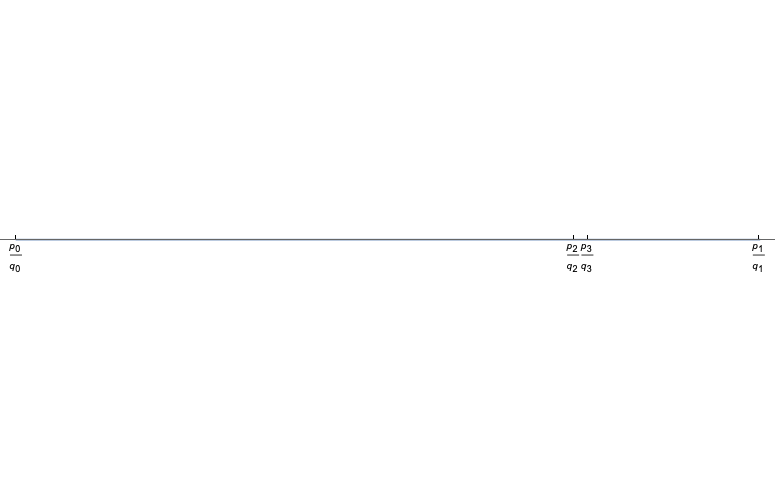
\includegraphics{example0}
\end{image}
\end{example}

\begin{example}
 Determine the continued fraction expansion and convergents for $\frac{5}{14}$
 
\begin{align*}
 \frac{5}{14}&=\answer{0}+\cfrac{1}{\answer{\cfrac{14}{5}}}
 =\answer{0}+\cfrac{1}{\answer{2}+\cfrac{1}{\answer{\cfrac{5}{4}}}}
 =\answer{0}+\cfrac{1}{\answer{2}+\cfrac{1}{\answer{1}+\cfrac{1}{\answer{4}}}}
\end{align*}
\begin{align*}
 \frac{p_0}{q_0}&=\frac{0}{1}, \frac{p_1}{q_1}=\frac{\answer{1}}{\answer{2}}, \frac{p_2}{q_2}=\frac{\answer{1}}{\answer{3}},\frac{p_3}{q_3}=\frac{\answer{5}}{\answer{14}}
\end{align*}
Here is a plot of the convergents
\begin{image}
 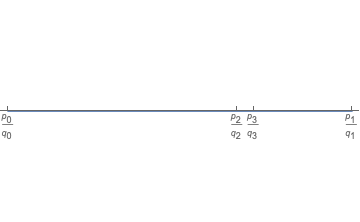
\includegraphics{example1}
\end{image}
\end{example}

\begin{example}
 Now we do our first example of an irrational number, the golden ration $G=\varphi=\frac{1+\sqrt{5}}{2}$. Now, $G$ is a root of $\answer{x^2-x-1}$, so $G=1+\frac{1}{G}$ (check for yourself). Substituting in for $G$, we get $G=1+\cfrac{1}{1+\cfrac{1}{G}}=[1;\overline{1}]$ where the $\overline{\cdot}$ indicates repeating digits, as with decimal expansions.
 
 Since every digit is $1$, this continued fraction expansion converges very slowly. Calculate a few of the convergents:
 \begin{align*}
  \frac{p_0}{q_0}&=\frac{1}{1}, \frac{p_1}{q_1}=\frac{\answer{2}}{\answer{1}},\frac{p_2}{q_2}=\frac{\answer{3}}{\answer{2}}, \frac{p_3}{q_3}=\frac{\answer{5}}{\answer{3}}, \frac{p_4}{q_4}=\frac{\answer{8}}{\answer{5}}\end{align*}
Here is a plot of the convergents
\begin{image}
 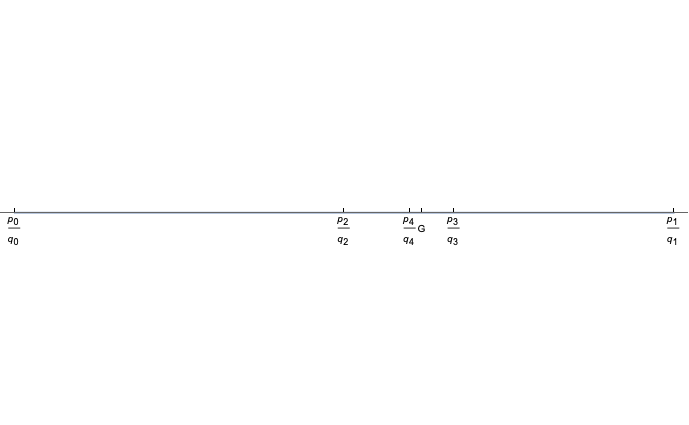
\includegraphics{example2}
\end{image}
\end{example}

Looking at all three plots, we can start to see that for $x\in\mathbb{R},x>0$, $\frac{p_0}{q_0}<x<\frac{p_1}{q_1}$ and $\frac{p_0}{q_0}<\frac{p_2}{q_2}<x<\frac{p_3}{q_3}<\frac{p_1}{q_1}$ (contrast this to the decimal expansion where $d_0\leq d_0.d_1\leq d_0.d_1d_2\leq d_0.d_1 d_2 d_3\leq\cdots$). In order to prove that this pattern continues (and holds for all positive real numbers), we need to prove a few more facts about $p_i$ and $q_i$.

\begin{theorem}
 Let $p_{-1}=1, q_{-1}=0, p_0=a_0, q_0=1$ (see that this matches with $p_0,q_0$ above). Then 
\begin{align}
 p_n&=a_np_{n-1}+p_{n-2}\label{pn}\\
 q_n&=a_nq_{n-1}+q_{n-2}\label{qn}
\end{align}
for $n\geq 1$.
\end{theorem}
\begin{proof}
 We start by checking $\frac{p_1}{q_1}=a_0+\frac{1}{a_1}=\frac{a_0a_1+1}{a_1}=\frac{p_0a_1+p_{-1}}{q_0a_1+q_{-1}}$. 
 
Next, we check $k=2$, $\frac{p_2}{q_2}=a_0+\cfrac{1}{a_1+\cfrac{1}{a_2}}=a_0+\frac{a_2}{a_2a_1+1}=\frac{a_0(a_2a_1+1)+a_2}{a_2a_1+1}=\frac{a_2p_1+p_0}{a_2q_1+q_0}$. 

 Now we proceed by induction. Assume that these recurrence relations hold for $n\leq k$. Then \[\frac{p_k}{q_k}=[a_0;a_1,a_2,\dots,a_k]=\frac{a_k p_{k-1}+p_{k-2}}{a_k q_{k-1}+q_{k-2}.}\]
 By definition, 
\begin{align*}
 \frac{p_{k+1}}{q_{k+1}}&=[a_0;a_1,a_2,\dots,a_k,a_{k+1}]=[a_0;a_1,a_2,\dots,a_k+\frac{1}{a_{k+1}}]\\
&=\frac{\left(a_k+\frac{1}{a_{k+1}}\right)p_{k-1}+p_{k-2}}{\left(a_k+\frac{1}{a_{k+1}}\right) q_{k-1}+q_{k-2}} \textrm{(by induction hypothesis*)}\\
&=\frac{{a_{k+1}}\left(a_kp_{k-1}+p_{k-2}\right)+p_{k-1}}{a_{k+1}\left(a_kq_{k-1}+{q_{k-2}}\right) +q_{k-1}}\\
&=\frac{{a_{k+1}}p_k+p_{k-1}}{a_{k+1}q_k +q_{k-1}}\textrm{(by induction hypothesis)}
\end{align*}
\end{proof}
*Often the recurrence relations \eqref{pn} and \eqref{qn} are proven using matrix multiplication instead of justifying that it is ok to substitute $a_k+\frac{1}{a_{k+1}}$ for $a_k$. The matrix definition also allows us to prove the next theorem by taking determinants. Instead, we will use induction and the recurrence relations.

\begin{theorem}
 For all $n\geq 1$, $p_nq_{n-1}-p_{n-1}q_n=(-1)^{n-1}$, which is equivalent to $\frac{p_n}{q_n}=\frac{(-1)^{n-1}}{q_nq_{n-1}}+\frac{p_{n-1}}{p_{n-1}}$.
\end{theorem}
\begin{proof}
The second equation is the first equation rewritten.

 We start with $i=1$, so from the previous theorem $p_1q_0-p_0q_1=(a_0a_1+1)1-a_0a_1=1=(-1)^0$.
 
 Now we proceed by induction. Assume that these recurrence relations hold for $n\leq k$. Then $p_kq_{k-1}-p_{k-1}q_k=(-1)^{k-1}$.
 Substituting in the recurrence relations  \eqref{pn} and \eqref{qn}, we get 
\begin{align*}
 p_{k+1}q_{k}-p_{k}q_{k+1}&=(a_{k+1}p_k+p_{k-1})q_k-p_k(a_{k+1}q_k +q_{k-1})\\
 &=p_{k-1}q_k-p_kq_{k-1}\\
 &=-(p_kq_{k-1}-p_{k-1}q_k)\\
 &=-(-1)^{k-1}=(-1)^k\qedhere
\end{align*}
\end{proof}

Notice that $\frac{p_n}{q_n}=\frac{(-1)^{n-1}}{q_nq_{n-1}}+\frac{p_{n-1}}{p_{n-1}}$ is still a recurrence relation. Expanding this out, we get \[\frac{p_n}{q_n}=a_0+\frac{1}{q_0q_1}-\frac{1}{q_1q_2}+\cdots+\frac{(-1)^{n-1}}{q_nq_{n-1}}=a_0+\sum_{k=1}^n\frac{(-1)^{k-1}}{q_{k-1}q_k}.\] Thus $x=\lim_{n\to\infty}\frac{p_n}{q_n}=a_0+\lim_{n\to\infty}\sum_{k=1}^n\frac{(-1)^{k-1}}{q_{k-1}q_k}=a_0+\sum_{k=1}^\infty\frac{(-1)^{k-1}}{q_{k-1}q_k}$ which converges by the alternating series test. This shows that the continued fraction expansion of $x$ really does converge to $x$ for all $x\in\mathbb{R},x>0.$

\begin{theorem}
 For $x\in\mathbb{R},x>0$, $\frac{p_0}{q_0}<\frac{p_2}{q_2}<\cdots<x<\cdots<\frac{p_3}{q_3}<\frac{p_1}{q_1}.$
\end{theorem}
\begin{proof}
From \eqref{qn}, we find that $q_0<q_1<q_2<\cdots$, since we have a recurrence relation that add positive integers to get a larger positive integer. Thus $\frac{1}{q_{n+1}q_n}<\frac{1}{q_nq_{n-1}}$.

For $n=2k$, we have that \begin{align*}\frac{p_{2k}}{q_{2k}}&=\frac{(-1)^{2k-1}}{q_{2k}q_{2k-1}}+\frac{p_{2k-1}}{p_{2k-1}}=\frac{-1}{q_{2k}q_{2k-1}}+\frac{(-1)^{2k-2}}{q_{2k-1}q_{2k-2}}+\frac{p_{2k-2}}{p_{2k-2}}\\
&=\frac{-1}{q_{2k}q_{2k-1}}+\frac{1}{q_{2k-1}q_{2k-2}}+\frac{p_{2k-2}}{p_{2k-2}},\end{align*}
and $\frac{-1}{q_{2k}q_{2k-1}}+\frac{1}{q_{2k-1}q_{2k-2}}>0$, so $\frac{p_0}{q_0}<\frac{p_2}{q_2}<\cdots<\frac{p_{2k}}{q_{2k}}<\cdots$. We also have that $\lim_{k\to\infty}\frac{p_{2k}}{q_{2k}}=x$ (from analysis) $\frac{p_0}{q_0}<\frac{p_2}{q_2}<\cdots<\frac{p_{2k}}{q_{2k}}<\cdots<x.$

For $n=2k+1$, we have that \begin{align*}\frac{p_{2k+1}}{q_{2k+1}}&=\frac{(-1)^{2k}}{q_{2k+1}q_{2k}}+\frac{p_{2k}}{p_{2k}}=\frac{1}{q_{2k+1}q_{2k}}+\frac{(-1)^{2k-1}}{q_{2k}q_{2k-1}}+\frac{p_{2k-1}}{p_{2k-1}}\\
&=\frac{1}{q_{2k+1}q_{2k}}+\frac{-1}{q_{2k}q_{2k-1}}+\frac{p_{2k-1}}{p_{2k-1}},\end{align*}
and $\frac{1}{q_{2k+1}q_{2k}}+\frac{-1}{q_{2k}q_{2k-1}}<0$, so $\cdots<\frac{p_{2k-1}}{q_{2k-1}}<\frac{p_{2k+1}}{1_{2k+1}}\cdots<\frac{p_{3}}{q_{3}}<\frac{p_1}{q_1}$. We also have that $\lim_{k\to\infty}\frac{p_{2k+1}}{q_{2k+1}}=x$ (from analysis) $x<\cdots<\frac{p_{2k-1}}{q_{2k-1}}<\frac{p_{2k+1}}{1_{2k+1}}\cdots<\frac{p_{3}}{q_{3}}<\frac{p_1}{q_1}.$
\end{proof}
\end{document}